\chapter{Running}

\section{How to install}

No installation is required. Once you unzip the PET file, \PET only requires a recent version of the Java Virtual Machine (\verb!1.6.0_26! or superior), which is likely to be already installed if you keep your machine up to date. 

On Microsoft Windows it is important to check whether the PATH to the Java binary files is properly set. Again, this may be already set. If you try to run the tool \ref{run} and it does not work, follow the guidelines in Section \ref{sec:win} to set the path.

\subsection{Windows}\label{sec:win}

\begin{enumerate}
	\item Do I have the right JVM?
	\begin{enumerate}
		\item Open a terminal
		\begin{figure}[H]\label{fig:terminal}
		\centering
		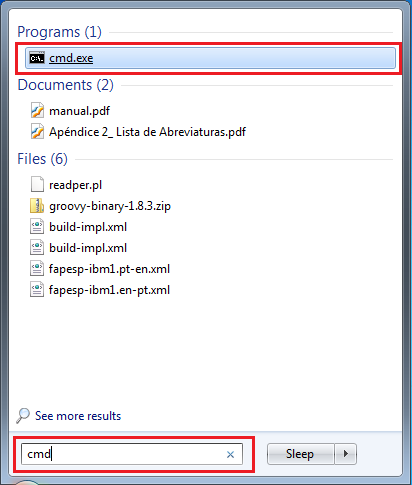
\includegraphics[width=0.5\textwidth]{img/step-by-step-win/1-open-cmd}
		\caption{Terminal}
		\end{figure}
		
		\item Type in {\tt java -version}
		\begin{figure}[H]\label{fig:version}
		\centering
		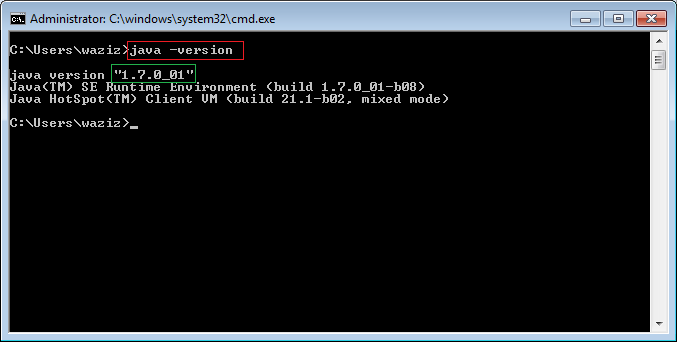
\includegraphics[width=0.75\textwidth]{img/step-by-step-win/2-java-version}
		\caption{Java version}
		\end{figure}
		
	\end{enumerate}
	
	\item What if my computer does not recognize the command {\tt java}?
	\begin{enumerate}
		\item Make sure you have downloaded and installed the JVM(\url{http://java.com/en/download/index.jsp}). 
	\end{enumerate}
	
	\item I am sure I have installed the JVM, yet I don't get it working, what can I do?
	\begin{enumerate}
		\item Open your computer's properties
		\begin{figure}[H]\label{fig:properties}
		\centering
		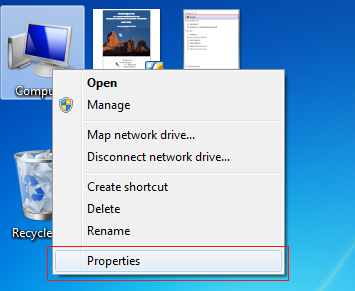
\includegraphics[width=0.5\textwidth]{img/step-by-step-win/3-computer-properties}
		\caption{Properties}
		\end{figure}
		
		\item Open the `Advanced Settings'
		\begin{figure}[H]\label{fig:advanced-settings}
		\centering
		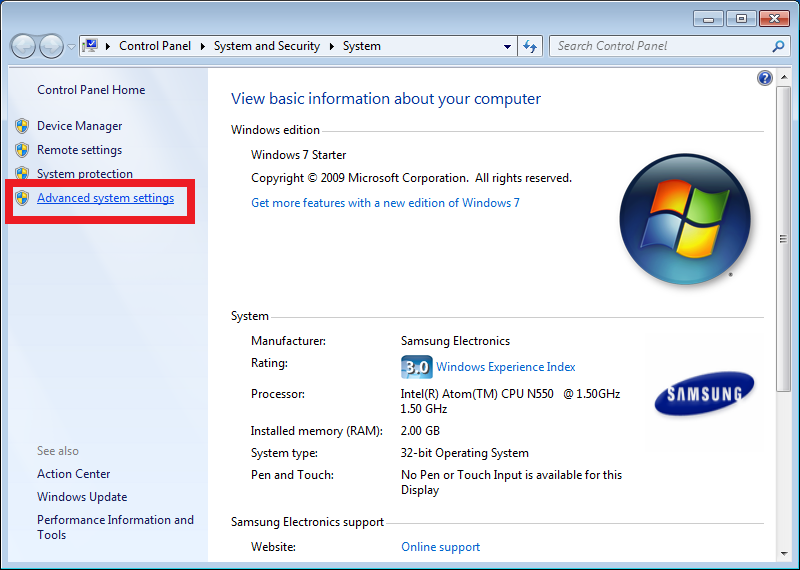
\includegraphics[width=0.5\textwidth]{img/step-by-step-win/4-advanced-settings}
		\caption{Advanced settings}
		\end{figure}
		
		\item Go to `Environment variables'
		\begin{figure}[H]\label{fig:variables}
		\centering
		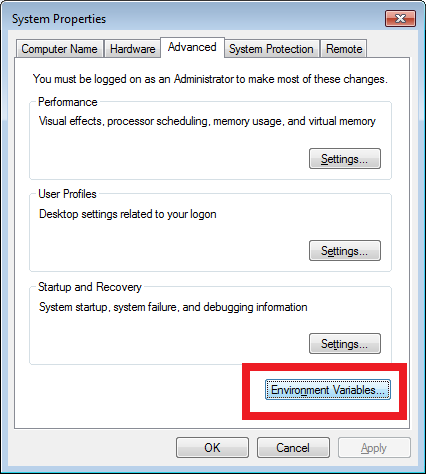
\includegraphics[width=0.5\textwidth]{img/step-by-step-win/5-environment-variables}
		\caption{Environment variables}
		\end{figure}
		
		\item Add a new variable
		\begin{figure}[H]\label{fig:newvar}
		\centering
		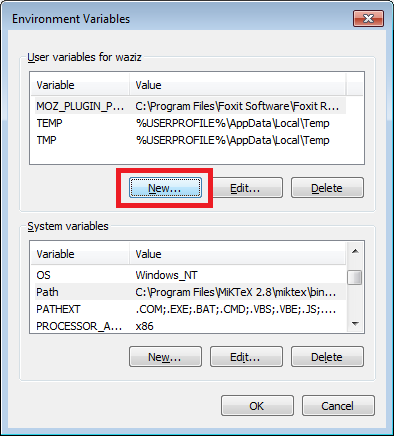
\includegraphics[width=0.5\textwidth]{img/step-by-step-win/6-new-variable}
		\caption{New user variable}
		\end{figure}
		
		\item Set variable's name and value to `PATH' and `$<$path-to-java$>$' respectively
		\begin{figure}[H]\label{fig:path}
		\centering
		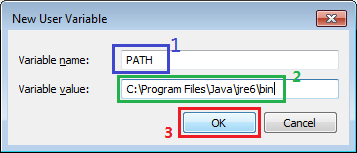
\includegraphics[width=0.5\textwidth]{img/step-by-step-win/7-set-path}
		\caption{Java's path}
		\end{figure}
		
		\item Conclude
		\begin{figure}[H]\label{fig:conclude}
		\centering
		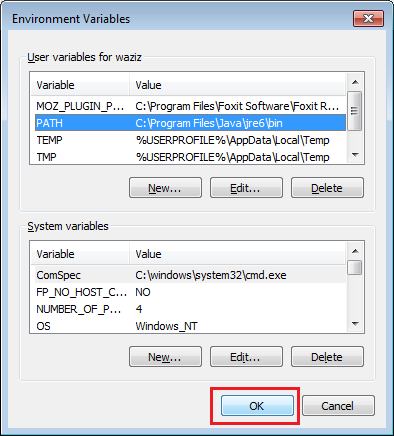
\includegraphics[width=0.4\textwidth]{img/step-by-step-win/8-conclude-1}
		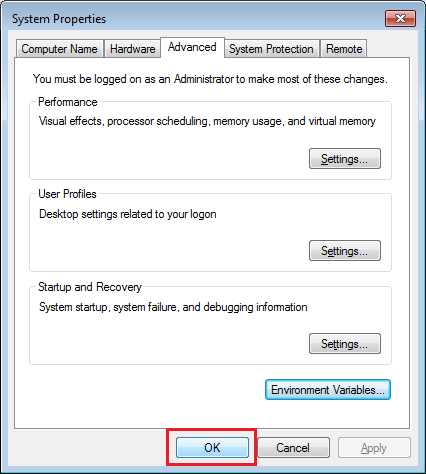
\includegraphics[width=0.4\textwidth]{img/step-by-step-win/8-conclude-2}
		\caption{Conclude}
		\end{figure}
	\end{enumerate}
	
	\item How do I find the path to Java binaries?
	\begin{enumerate}
		\item Open a terminal (see Figure \ref{fig:terminal})
		\item Type in {\tt where java}
		\begin{figure}[H]\label{fig:where}
		\centering
		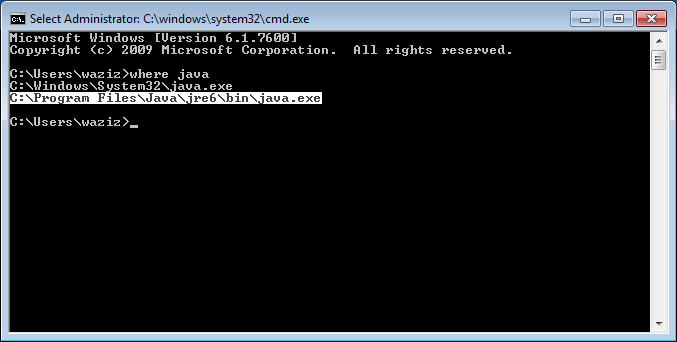
\includegraphics[width=0.75\textwidth]{img/step-by-step-win/0-0-localize-java}
		\caption{Finding Java}
		\end{figure}
		
		If this does not work you may try the following:
		
		\item Open the Windows Explorer (e.g. double click `Computer')
		\item Find the directory where you have installed Java (usually \verb!C:\Program Files\Java!)
		\item Go to \verb!jre6\bin!
		\begin{figure}[H]\label{fig:jre}
		\centering
		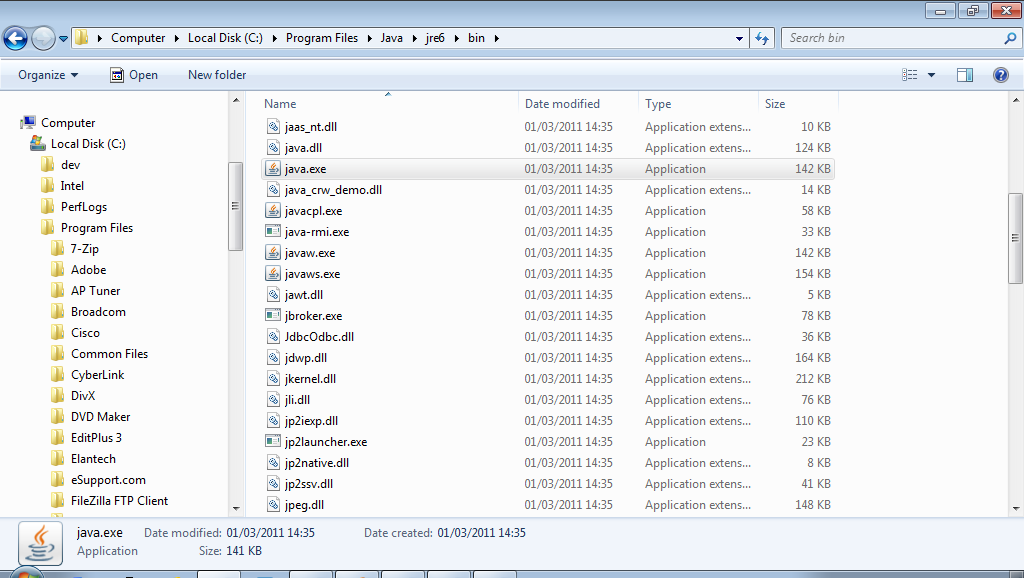
\includegraphics[width=1.0\textwidth]{img/step-by-step-win/0-1-localize-java}
		\caption{Java installation folder}
		\end{figure}
		\item Copy the path from the address bar
		\begin{figure}[H]\label{fig:address}
		\centering
		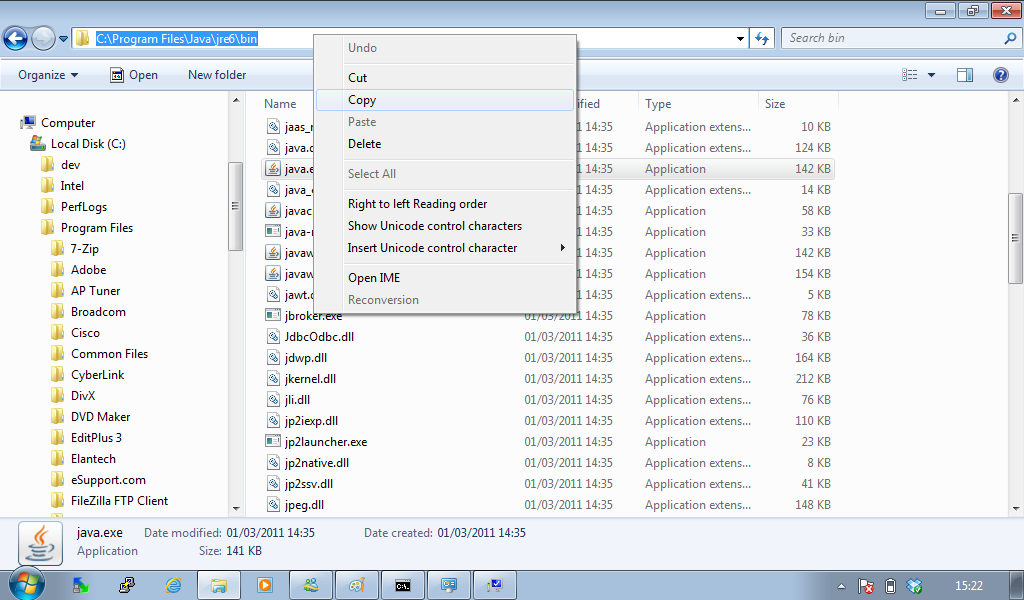
\includegraphics[width=1.0\textwidth]{img/step-by-step-win/0-2-copy-path}
		\caption{Path to binaries}
		\end{figure}
	\end{enumerate}
	
\end{enumerate}


\section{How to run}\label{run}

Simply execute the file {\tt run.bat}.
On Windows double clicking the file will be enough.
On Linux or Mac if the ``executable permission'' is set, double-clicking the file then selecting ``run on terminal'' will be enough. If not, set it under the tab ``Permissions'' right-clicking the file, or open a terminal and type {\tt sh run.bat}.